% two ways to ciet:
%  \textcite{label}
%  \parencite{label}

UAVs have been widely used for personal, commercial,
industrial, academic, and military purposes.
In many situations, they provide flexible and cost-effective solutions.
For example, first-person view (FPV) drones are widely used by video bloggers,
and surveillance drones greatly promote intelligence capabilities of an army.

However, the use of a single UAV is limited by its size,
sensors, computing power, and other hardware restrictions.
Besides, once a single UAV fails, the task being executed by it will also fail.
In recent years, with the advancement of technology,
it has become possible to group multiple UAVs into a swarm to perform complex tasks.
Compared to single UAVs, swarms feature the advantages of high efficiency and robustness,
and significantly expand the ways in which UAVs are used.
Many researchers have investigated the potential use cases
of swarms \parencite{Dimakos2024, Javaid2023, Ouyang2023, GAO2023, Zhou2020}.
In civilian fields, swarms can contribute to large-scale environmental monitoring,
efficient post-disaster search and rescue, forest fire fighting, logistics, etc.
In military fields, swarms may be used to enhance reconnaissance,
or even aerial warfare.

It should be noted that, a ``swarm" in this thesis refers to a group of UAVs
which autonomously coordinate with each other in real-time to complete tasks.
If the UAVs in a group just fly and operate according to preprogrammed data,
of if the UAVs are fully controlled by a remote control centre, e.g., a GCS,
then the UAV group is not considered a swarm.

Generally, for a single UAV,
the onboard hardware and software may include the following functionalities.
\begin{itemize}
    \item Communication:
    A UAV needs to exchange data with other UAVs or with a ground control station (GCS).
    \item Environment perception:
    A UAV needs to detect obstacles and to track targets.
    It also needs positioning information, which may come from a GPS receiver.
    \item Path planning:
    The flight path shall meet the requirement of a certain task.
    Collision with obstacles or other UAVs must be avoided.
    \item Flight control:
    With planned flight path, the actuators and engines shall be controlled
    according to aerodynamic principles, so as to acquire desired attitude and velocity.
    \item Task planning:
    When assigned a task, e.g., delivering a parcel,
    a UAV needs to figure out how to accomplish it.
    This is especially important for an autonomous UAV.
\end{itemize}
For a UAV swarm, except for all the above technical difficulties for single UAVs,
there are also additional challenges including
but not limited to \parencite{Javed2024, Zhou2020, Brambilla2013}:
\begin{itemize}
  \item Network topology
  \parencite{Javed2024, Javaid2023, Chen2020, Campion2019, Brust2015}:
  In some cases, the communication among UAVs is limited by a lot of factors,
  such as communication range, bandwidth, obstacles and terrain.
  An all-to-all communication network may not be feasible.
  Therefore, a good network topology design is needed to ensure efficient data transfer.
  \item Formation control
  \parencite{Javed2024, Wan2023, Ouyang2023, Shahzad2023, Ma2022, Kamel2020}:
  UAVs need to stay together to form a swarm.
  In some cases, the UAVs also need to maintain their relative positions inside a swarm.
  \item Path planning
  \parencite{Javed2024, Dimakos2024, PuenteCastro2022}:
  For swarms, the fight path needs to be planned with a view of the entire swarm.
  Besides, flight path of each individual UAV is closely coupled with
  the formation control and network topology of the whole swarm.
  \item Task planning and allocation
  \cite{Cao2024, Javed2024, Li2023, Peng2021, Ma2022}:
  The task of the whole swarm must be planned and
  divided into sub-tasks for each individual UAV.
  For most UAV tasks, task management may overlap with path planning and
  formation maintaining to some extent. For instance, in aerial search tasks,
  flight path must ensure coverage of target areas.
  While in drone shows, the task itself is to form certain formations.
\end{itemize}
To fully explore and utilise UAV swarms,
a lot of algorithms have been developed regarding different aspects of swarms.
This thesis will particularly focus on formation control and task allocation.

\section{Formation Control}

For a swarm to function normally, UAVs need to stay close to each other,
in order to communicate and cooperate.
For certain tasks, UAVs are even required to keep rigid relative positions.
Since swarm formation is ultimately achieved by the movement of every individual UAV,
formation control is therefore closely coupled with path planning.
In this section, some popular algorithms related to
formation control and path planning are reviewed.

\subsection{Leader-follower Method}

In the leader-follower method \parencite{Ouyang2023, Wan2023, Kamel2020},
one UAV is chosen as the leader, while all other UAVs are followers.
The leader is responsible for calculating the flight path.
The followers just track and follow the leader.
This method is simple to implement.
Especially for the followers,
the formation problem is converted into a trajectory tracking problem.
However, swarms employing this method risk single points of failure.
As the leader UAV acts as a central control node,
once it breaks down, the whole swarm may malfunction.
Moreover, the calculation of the swarm flight path is done by the leader alone,
which may pose a huge burden for its computing resource.

\subsection{Virtual Structure Method}

The virtual structure method treats the desired formation as a rigid virtual structure
\parencite{Ouyang2023, Wan2023, Kamel2020}.
Each UAV is expected to embody a respective virtual point on the virtual rigid body.
It observes the positions and velocities of other UAVs,
fits the position, orientation, and velocity of the virtual structure,
and then calculates its appropriate position and velocity.
There is no central UAV,
but the virtual geometric centre can be viewed as the leader of the swarm,
and all the UAVs follow this virtual leader,
as depicted by figure \ref{fig:virtual_structure}.
Therefore this method is also known as virtual leader method.

\begin{figure}[htbp]
  \centering
  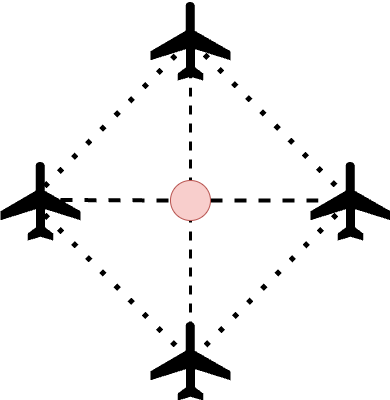
\includegraphics[width=0.4\linewidth]{rsc/virtual_structure_method.png}
  \caption[Virtual structure method.]
  {In virtual structure method, the UAVs can be viewed as
  following the virtual geometric centre.}
  \label{fig:virtual_structure}
\end{figure}

Due to the elimination of a central node, the virtual structure method is robust.
But the UAVs are required to maintain a rigid formation,
this compromises flexibility in some cases, e.g., when avoiding obstacles.

\subsection{Behaviour-based Method}

Inside a swarm, each UAV may have several prescribed basic behaviours.
For eaxample, aggregation, separation, collision avoidance, and target tracking.
Each behaviour calculates a desired velocity according to some rule.
A coordinator is responsible for synthesising the final velocity out of these
behavioural velocities, based on information from the environment and other UAVs.

One of the velocity synthesis methods is the null-space
method \parencite{Arrichiello2010, Falconi2008, Antonelli2005, Bishop2001}.
Each basic behaviour is assigned a priority.
Velocity vector of lower-priority is projected onto the null space
of the immediately higher-priority velocity, as shown in figure \ref{fig:null_space}.
In this way, lower-priority behaviour will not conflict with higher-priority behaviour.

\begin{figure}[htbp]
  \centering
  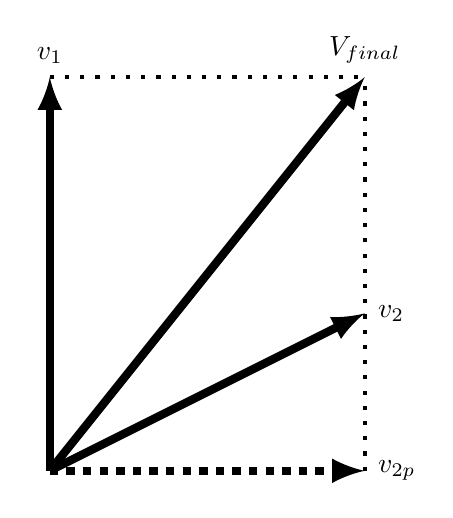
\begin{tikzpicture}
    \draw[line width=3pt,black,-latex](0,0)--(0,5) node[anchor=south]{$v_1$};
    \draw[line width=3pt,black,-latex](0,0)--(4,2) node[anchor=west]{$v_2$};
    \draw[line width=3pt,black,dashed,-latex](0,0)--(4,0) node[anchor=west]{$v_{2p}$};
    \draw[line width=1.5pt,black,loosely dotted](4,0)--(4,5);
    \draw[line width=1.5pt,black,loosely dotted](0,5)--(4,5);
    \draw[line width=3pt,black,-latex](0,0)--(4,5) node[anchor=south]{$V_{final}$};
  \end{tikzpicture}
  \caption[Null-space method.]
  {In null-space method, the velocity $v_2$ from the lower-priority behaviour
  is projected onto the null space of the higher-priority $v_1$,
  resulting in $v_{2p}$, and the final velocity is $V_{final} = v_1 + v_{2p}$.}
  \label{fig:null_space}
\end{figure}

Behaviour-based method can be used not only in UAV swarm
formation control and path planning, in fact, it can be viewed as a
general framework for coordinating interacting behaviours \parencite{Kamel2020}.
The behaviour coordination mechanism is at the core of this method.
For the case of formation control, behaviour coordination means velocity synthesis.

\subsection{Bio-inspired Methods and Other Methods}

Bio-inspired methods draw ideas from natural swarm behaviours,
especially biological phenomena.
For example, many bird species fly in flocks,
so if UAVs imitate the behaviours of birds, UAV swarms may display similarities to
bird flocks \parencite{Ma2022, Reynolds1987}.
Another interesting example is morphogenesis approach \parencite{Ma2022, MAMEI2004}.
Morphogenesis, i.e., the formation of the shape of organs,
is connected with signal molecules that diffuse among cells, also known as morphogen.
Cells adjust their behaviour according to the concentration of morphogen,
and eventually the organ will develop a certain shape.
Inside a swarm, messages can be propagated in certain pattern between neighbouring UAVs.
If all UAVs act properly according to these messages,
the swarm will be able to develop a global shape in a self-organised way.

There are also many other types of formation control methods,
such as artificial intelligence (AI) methods \parencite{PuenteCastro2022},
artificial potential fields \parencite{Shahzad2023, Wang2006, Schneider2003},
graph-based(consensus-based) algorithms \parencite{Ouyang2023, Kamel2020},
and so on.

\section{Task Allocation}

However, for an autonomous swarm,
it is equally crucial to optimally schedule tasks and allocate them to individual UAVs.
Usually, for UAV, task management is highly related to path planning,
after all, most tasks have restrictions on the position and velocity of a UAV.
Moreover, in real scenarios, resources such as fuel or power are constrained for a task,
making the problem even harder to tackle \parencite{Javed2024, Zhou2020}.

One relatively easy way to manage swarm tasks is to take a centralised approach.
That is, one UAV works as a central node, schedules tasks and allocates them to others.
However, due to single points of failure, this method is not robust.
Decentralised methods, where every UAV takes part in the task allocation process,
are more resilient but also more complex.
Many algorithms have been studied for their usage
in swarm task allocation \cite{Peng2021, Plathottam2018},
such as game theory, reinforcement learning, etc.
In this section, some of them are reviewed.

\subsection{Algorithms Based on Market Mechanisms}

These algorithms imitate marketing processes.
A typical example is the auction algorithm \parencite{Peng2021, Kim2020, Sujit2007}.
If a UAV has a task, but does not own the requisite resource,
it can choose to auction the task.
Other UAVs can bid, and the winner is assigned the task.
Auction algorithm has clear rules and is easy to perform.
It requires good communication between the auctioneer and the bidders.

\subsection{Consensus-based Methods}

In consensus methods, if a UAV wants to take any action,
or if it wants the whole swarm to take any action,
it firstly negotiates with other UAVs,
and they need to reach an agreement on whether or not the action should be taken.
If consensus is reached, the action will be taken,
otherwise the action is abandoned.
It can be seen that consensus algorithms require good communication inside the swarm.
Many researchers have studied different types of consensus methods and
their variants \parencite{Pasek2022, Ranganathan2022, Grishchenko2021, Li2019}.
The difficult part of a consensus algorithm is for a UAV to decide
whether all others have been informed of and have agreed on its proposal,
especially in real-world scenarios where network topology is constrained
and communication condition is not ideal.

Consensus algorithms have a wide range of applications.
They can be used not only in swarm task allocation,
but also in formation control, path planning,
and many other types of distributed systems,
e.g., a distributed software system \parencite{Ongaro2014}.

\subsection{Optimisation Algorithms}

Since time and resources are limited for a swarm,
optimisation algorithms come into play,
so as to plan and allocate tasks in a most optimal way.
Note that, optimisation is not used for
reaching an agreement on which UAV takes which sub-task,
but for finding out the best task division scheme.

A particular type of optimisation methods are swarm intelligence algorithms
\parencite{Cao2024, Javed2024, Tang2023, Peng2021, Zhou2020, Tan2013, Beni1993}.
Swarm intelligence is not a strict term,
but a loose concept that solves problems by modelling a population of agents
which can self-organise and interact with each other.
After a population is set to some initial state,
each individual agent acts by certain principle,
eventually, the whole population may achieve specific collective behaviour
or reach desired global optimum state.
A lot of swarm intelligence methods are inspired by biological swarm behaviours.
Swarm intelligence can be used in many problems, and optimisation is just one of them.
Some common swarm intelligence optimisation algorithms are genetic algorithm (GA),
particle swarm optimisation (PSO) \parencite{Bonyadi2017, Duan2013, Roberge2013},
ant colony optimization (ACO),
wolf pack algorithm (WPA) \parencite{Xu2022, Lu2020},
and so on.

\section{Hierarchical Swarm}

Despite of lot of research effort put into UAV swarms,
they are still not mature for real-world applications.
In 2021, \textcite{Lee2021} reported an experiment where
3 UAVs planned their flight path to avoid no-fly zones and
kept their formation with leader-follower method.
In 2016, US department of defense conducted a micro-drone swarm test \parencite{DOD2017}.
In the test, 103 small drones were launched from fighter jets.
The drones demonstrated collective decision making,
adaptive formation flying, and other swarm behaviours.
However, technical details were not disclosed.
In 2022, British Army carried out a demonstration where
swarms comprised of 4 or 6 drones executed autonomous missions \parencite{BA2022}.
Again, no technical details.
As can be seen from the above examples,
current swarms are either quite small, or can only deal with simple tasks.
This is not surprising since swarm algorithms are still in their early stage.

\subsection{Drawbacks of Common Algorithms}

Swarm control algorithms can be roughly divided into two categories,
centralised ones and decentralised ones.
Centralised algorithms usually have a leader UAV as a central node,
whereas all other UAVs are managed by the leader.
The leader-follower formation control method is an example of centralised algorithm.
Such algorithms are simple and efficient,
but are vulnerable to single points of failure.
Besides, as most computation happens on the central node,
it usually needs much more communication and computing power than others.
Therefore the swarm size may be limited by the resource on the central node.
In contrast, decentralised algorithms treat every UAV equally,
and the collective behaviour of the whole swarm is coordinated by all the UAVs involved.
Such algorithms are more robust.

In this thesis, decentralised algorithms are further divided into two types.
The first type is negotiation-based ones,
such as auction algorithms and consensus algorithms.
UAVs communicate with each other about what they plan to do next,
and make decisions together.
Consensus algorithms are powerful,
because each UAV knows what others will do,
and they have a fine control on task management.
However, they impose a high communication and computation burden on swarms,
since every UAV cares for the whole swarm.
As swarm population increases,
the complexity of communication and control goes up sharply.
Thus, the swarm size is limited.

Another type of decentralised algorithms is reaction-based ones,
such as virtual structure formation control, and most bio-inspired algorithms.
In these algorithms, UAVs do not need to reach agreement.
They just gather information about the environment and other UAVs,
then they react according to preset rules.
Such algorithms are highly robust,
and do not require much communication or computation resource.
They are highly distributed and suitable for large swarms.
However, they lack fine and flexible control over the swarm,
hence are not versatile and are only adequate for simple tasks.
Table \ref{tbl:algorithms_cmp} shows a comparison between different types of algorithms.

\begin{table}[htbp]
\centering
\caption[Comparison of swarm algorithms.]
{Comparison of different types of swarm algorithms.}
\label{tbl:algorithms_cmp}
\begin{tabular}{|c||c|c|c|}
  \hline
  Algorithm Type       & Centralised         & Negotiation-based & Reaction-based \\
  \hline\hline
  Robustness           & not robust          & robust            & robust         \\
  \hline
  Algorithm Complexity & simple              & complex           & intermediate   \\
  \hline
  Performance Overhead & high (central node) & high (all nodes)  & low            \\
  \hline
  Supported Tasks      & complex             & complex           & simple         \\
  \hline
  Supported Swarm Size & small               & small             & large          \\
  \hline
\end{tabular}
\end{table}

\subsection{A Hierarchical Method}

This thesis aims to find an algorithm that is robust, suitable for complex tasks,
adequate for large swarms, and low in performance overhead.
The solution is a hierarchical swarm.
The swarm is organised into a tree structure.
Each UAV corresponds to a node on the tree structure,
and it is in direct control of the UAVs which correspond to its child nodes.
Layer by layer, the root node will be controlling the whole swarm in an indirect way,
quite similar to the hierarchy in modern companies, governments, or armies.
Figure \ref{fig:swarm_tree} shows such an swarm structure.
Communication mainly happens between each parent-child node pairs.
For most of the time, there is no need for many-to-many communication,
reducing the communication overhead.
Task is also solved by hierarchical coordination.
A node receives task from its parent, then divides the task,
and assigns the sub-tasks to itself and its children.
The children then repeat the process.
This divide-and-conquer way of task coordination potentially reduces computing overhead.
As the tree grows in depth, the number of nodes grows exponentially,
therefore large swarm sizes are supported.

\begin{figure}[htbp]
  \centering
  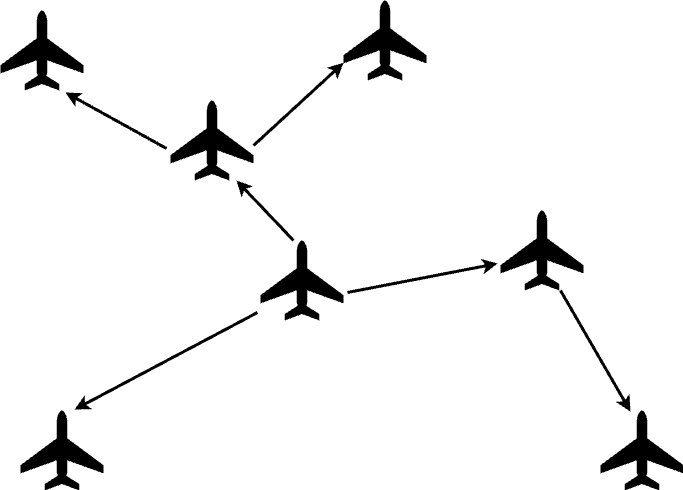
\includegraphics[width=0.4\linewidth]{rsc/swarm_tree.png}
  \caption[Hierarchical swarm.]
  {A swarm organised hierarchically into a three-layer tree.
  Arrows point from parent node to child node.}
  \label{fig:swarm_tree}
\end{figure}

Actually, researchers have already investigated the usage of hierarchical structure
in swarm organisation \parencite{CHEN2021, Wang2021, Tahir2020}.
In those researches, the hierarchy, which is not necessarily a tree,
is predefined and fixed before flight.
This leads to reduced flexibility and robustness.
In fact, a tree is just a multi-layered leader-follower structure, which is centralised.
To mitigate the disadvantages of leader-follower approach induced by centralisation,
some researchers have proposed dynamic leader election
algorithms \parencite{Ganesan2020, Brust2015}.
Similarly, to make the swarm tree structure flexible and robust,
it needs to be organised dynamically.
That is, the UAVs themselves build up the tree,
and they are able to repair the tree structure in case any of them fails.

In the next chapters, the algorithm for dynamic hierarchical swarm organisation
will be developed and implemented.
The task for the swarm is to form designated geometric shapes.
This application scenario is inspired by drone light shows \parencite{VergeAero}.
Currently, drone light shows do not employ autonomous UAV swarms.
But this thesis shows the possibility for their usage in the future.